\documentclass[12pt, legalpaper]{exam}
\usepackage[utf8]{inputenc}
\usepackage[english]{babel}
\usepackage[margin=.8in]{geometry}
\usepackage{amsmath,amssymb}
\usepackage{multicol}
\usepackage{graphicx}
\usepackage{tikz}
\usepackage{lastpage}
\usepackage{tabularx}
\usepackage{hyperref}
\usepackage{tcolorbox}
\newcommand{\course}{Introduction to Optimization}
\newcommand{\term}{Fall 2023}
\newcommand{\examnum}{Constructive Report on Programming Task 1}


\begin{document}
\noindent ''\course'' - \term

% \noindent Date: .............  


\noindent
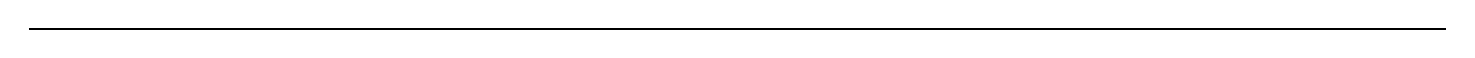
\begin{tikzpicture}
\draw[thick] (0,0) -- (18,0);
\end{tikzpicture}




\vspace{12pt}
\begin{center}
    \textbf{Constructive Report 1}
\end{center}
% \noindent \textbf{Requirements}

\vspace{12pt}

\noindent  \textbf{Team information.}

\begin{table}[h!]
    \centering
    \begin{tabular}{|m{7cm}|m{7cm}|}\hline
        \textbf{Report by} & \textbf{Product by} \\ \hline
    Team leader: Ilia Mitrokhin & Team leader: Alexey Tkachenko\\ 
    Team member 1: Max Martyshov&
    Team member 1: Alsu Khairullina\\
    Team member 2: Mintimer Karimov&
    Team member 2: Ekaterina Zaitseva\\
    Team member 3: Kirill Arkhipov&   
    Team member 3: Natalia Agapova\\
    Team member 4: Timur Zheksimbaev&
    Team member 4: Nika Chekhonina\\
    Team member 5: Aleksandr Ryabov&
    Team member 5: Timofey Ivlenkov \\ \hline
    \end{tabular}
    % \caption{Caption}
    % \label{tab:my_label}
\end{table}



\vspace{12pt}



\noindent
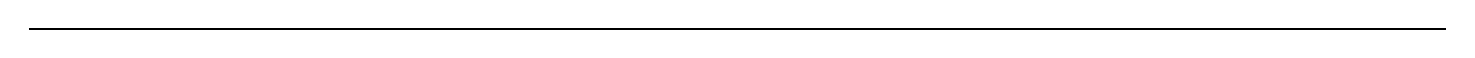
\begin{tikzpicture}
\draw[thick] (0,0) -- (18,0);
\end{tikzpicture}
\noindent     \textbf{General opinion}

\vspace{12pt}
\textbf{Format of product:}

The product is in the form of code and it is available as a git repository on the Github platform.

The product comes with documentation that describes the rules for working with Git,
building the program, and instructions on how to use it.

\vspace{12pt}
\textbf{Structure of product:}

The product is written in C++ and uses CMake with GCC to compile it.

Using the CMake build system is a good way: it simplifies
usage of the project and future improvements.

\vspace{6pt}

In products using the object-oriented paradigm of programming:
in one file it described work with matrices, in another file
the pure simplex algorithm and in the last one are both composed
with user input-output.

This programming paradigm improves scaleability and
reuseability of program code for the improvements.

\vspace{12pt}
\textbf{Algorithms using in product:}

Inside product implemented a standard simplex algorithm based on matrix operations.

Algorithms are specified in separate files and every operation separated from others,
that makes easier understanding of code.

\vspace{12pt}
\textbf{Summary:}

Totally, the quality of the product is high by all criteria: code structure, quality, and readability;
product usage is clear and simple for users;
simplex algorithm implemented properly well.


\vspace{2cm}
\noindent
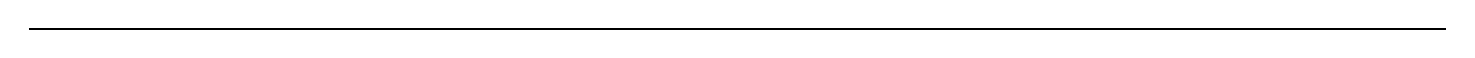
\begin{tikzpicture}
\draw[thick] (0,0) -- (18,0);
\end{tikzpicture}

\vspace{12pt}
\noindent     \textbf{Improvement}

\vspace{12pt}


For future improvements we can advise to add an example of input and output,
that makes simpler use of the product and allows user to check the result of program building.
\end{document}